% Copyright © 2015 Martin Ueding <dev@martin-ueding.de>

\documentclass[11pt, english, fleqn, DIV=15, headinclude, BCOR=1cm]{scrartcl}

\usepackage[bibatend, color]{../header}

\usepackage{tikz}

\usepackage[tikz]{mdframed}
\newmdtheoremenv[%
    backgroundcolor=black!5,
    innertopmargin=\topskip,
    splittopskip=\topskip,
]{theorem}{Theorem}[section]

\hypersetup{
    pdftitle=
}

\newcounter{totalpoints}
\newcommand\punkte[1]{#1\addtocounter{totalpoints}{#1}}

\newcounter{problemset}
\setcounter{problemset}{4}

\subject{Geometry in Physics}
\ihead{Geometry in Physics -- Problem Set \arabic{problemset}}

\title{Problem Set \arabic{problemset}}

\publishers{Group 1 -- Jens Boos}
\ofoot{Group 1 -- Jens Boos}

\author{
    Martin Ueding \\ \small{\href{mailto:mu@martin-ueding.de}{mu@martin-ueding.de}}
    \and
    Paul Manz \\ \small{\href{mailto:paul.manz@dreiacht.de}{paul.manz@dreiacht.de}}
}
\ifoot{Martin Ueding, Paul Manz}

\ohead{\rightmark}

\usepackage{multicol}

\renewcommand\thesubsection{\thesection.\alph{subsection}}

\begin{document}

\maketitle

\vspace{3ex}

\begin{center}
    \begin{tabular}{rrr}
        problem & achieved points & possible points \\
        \midrule
        \nameref{homework:1} & & \punkte{10} \\
        \nameref{homework:2} & & \punkte{10} \\
        \nameref{homework:3} & & \punkte{10} \\
        \nameref{homework:4} & & \punkte{20} \\
        \midrule
        Total & & \arabic{totalpoints}
    \end{tabular}
\end{center}

\section{Visualization of differential forms}
\label{homework:1}

\subsection{Visualization}

The forms can be visualized in the dual space. In the dual space, there should
not be a problem by visualizing them with vectors. Vectors are translationally
invariant, so we can draw them anywhere, just like it is done on the problem
set. All four forms are shown in Figure~\ref{fig:forms}.

\begin{figure}[htbp]
    \centering
    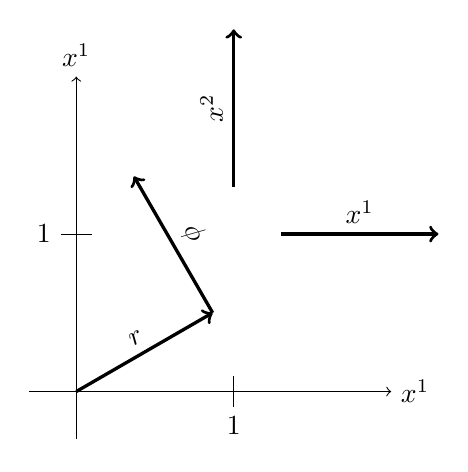
\begin{tikzpicture}[scale=2]
        \draw[->] (-.3, 0) -- (2, 0) node[right] {$\dif x^1$};
        \draw[->] (0, -.3) -- (0, 2) node[above] {$\dif x^1$};

        \draw (1, .1) -- (1, -.1) node[below] {$1$};
        \draw (.1, 1) -- (-.1, 1) node[left] {$1$};

        \draw[very thick, ->] (1.3, 1) -- ++(1, 0) node[midway, sloped, above] {$\dif x^1$};
        \draw[very thick, ->] (1, 1.3) -- ++(0, 1) node[midway, sloped, above] {$\dif x^2$};

        \draw[very thick, ->] (0, 0) -- ++(30:1) node[midway, sloped, above] {$\dif r$};
        \draw[very thick, ->] (30:1) -- ++(120:1) node[midway, sloped, above] {$\dif \phi$};
    \end{tikzpicture}
    \caption{%
        Visualization of $\dif x^1$, $\dif x^2$, $\dif r$ and $\dif \phi$ in
        the dual space.
    }
    \label{fig:forms}
\end{figure}

\paragraph{Transformation into Cartesian coordinates}

The forms given in polar coordinates have to be transformed into Cartesian
coordinates to draw them into the Cartesian plot. Although the representation
in Cartesian coordinates seems “obvious”, we would like to engage the full
machinery of pullbacks and pushforwards in order to see whether we understood
the concepts correctly.

So we have $\omega^3 = \dif r$ given. We write the index 3 as an upper index
since this 1-form itself has one lower covariant index. The transformation
which brings us from Cartesian to polar coordinates is given by
\begin{align*}
    \varphi \colon &\R^2_\text{Cartesian} \mapsto \R^2_\text{polar} \\
                &x \ev_x + y \ev_y \to \sqrt{x^2 + y^2} \, \ev_r + \arctan\del{\frac yx}
    \ev_\phi,
\end{align*}
although it is not well defined for all angles $\phi$. As long as we restrict
this to the first quadrant, everything is fine. Let us restrict this to the
open set $(0, \infty) \times (0, \infty)$ to make it easier. Then $\varphi$ is
a diffeomorphism.

Now we use a pullback which will let us bring tensors the other way around.
This is best expressed more formally:
\[
    \varphi^* \colon T_{\varphi(\xi)}\R^2_\text{polar} \mapsto T_{\xi}\R^2_\text{Cartesian}
\]
$\xi$ is a point given in Cartesian coordinates. The components of a tensor
$\tens\omega$ then transform like the following:
\[
    [\varphi^* \omega]^{\nu_1 \ldots}{}_{\mu_1\ldots}(\xi) =
    \omega^{\alpha_1 \ldots}{}_{\beta_1\ldots} (\varphi(\xi))
    \pd{y^{\beta_1}}{x^{\mu_1}} \cdots
    \pd{x^{\nu_1}}{y^{\alpha_1}} \cdots
    \eqnsep
    \vec y := \vec\varphi(\xi).
\]

With our given 1-form, this collapses to a single lower index:
\begin{align*}
    [\varphi^* \omega^3]_i(\xi)
    &= \omega^3_j(\varphi(\xi)) \pd{\varphi^j}{x^i}(\xi).
    \intertext{%
        $\omega$ is just $\dif r$, so we have the components $\omega_r = 1$ and
        $\omega_\phi = 0$. $r$ is not an index which takes on numbers, but we
        rather want it to be interpreted that $j \in \{r, \phi\}$. This is a
        bad overloading of symbols, but we hope that it is somewhat
        decipherable. Since there is only one component in $\omega$ the
        equation simplifies to
    }
    &= 1 \cdot \pd{\varphi^r}{x^i}(\xi).
    \intertext{%
        Using the explicit form of the map $\vec \varphi$, the partial
        derivatives are
    }
    &= \sbr{\frac{x_i}{\sqrt{x^2 + y^2}}}_{\xi}.
\end{align*}
This is now expressed in terms of Cartesian coordinates. It simplifies
to use the polar coordinates to write this more compact. Then we have
\[
    [\varphi^* \omega^3]_i \dif x^i
    = \omega^3
    = \cos(\phi) \dif x + \sin(\phi) \dif y.
\]

This result seems “obvious” but this derivation should hold for arbitrary
diffeomorphisms.

\subsection{Value of forms on vectors}

The vectors given in the image are:
\[
    \vec v_1 = \begin{pmatrix} 0 \\ 1 \end{pmatrix}
    \eqnsep
    \vec v_2 = \begin{pmatrix} -1 \\ -1 \end{pmatrix}
    \eqnsep
    \vec v_3 = \begin{pmatrix} 1 \\ -1 \end{pmatrix}
\]

Everything is summarized in Table~\ref{tab:values}.

\begin{table}[htbp]
    \centering
    \begin{tabular}{c|ccc}
        & $\vec v_1$ & $\vec v_2$ & $\vec v_3$ \\
        \midrule
        $\omega_1$ & 0 & & \\
        $\omega_2$ & & & \\
        $\omega_3$ & & & \\
    \end{tabular}
    \caption{%
        Summary of value of the forms on the vectors.
    }
    \label{tab:values}
\end{table}

\section{Straight forward calculations}
\label{homework:2}

\section{Hyperbolid coordinates}
\label{homework:3}


\section{Pullback}
\label{homework:4}



\end{document}

% vim: spell spelllang=en tw=79
